

%----------
% DOCUMENT CONFIGURATION
%----------

\documentclass[12pt]{report} %font 12pt

% MARGINS
\usepackage[
a4paper,
vmargin=2.5cm,
hmargin=3cm
]{geometry}

\renewcommand{\baselinestretch}{1.15}
\parskip=6pt

% COLORS for cover and code
\usepackage[table]{xcolor}
\definecolor{azulUC3M}{RGB}{0,0,102}
\definecolor{gray97}{gray}{.97}
\definecolor{gray75}{gray}{.75}
\definecolor{gray45}{gray}{.45}

% Soporte para GENERAR PDF/A --es importante de cara a su inclusión en e-Archivo porque es el formato óptimo de preservación y a la generación de metadatos, tal y como se describe en http://uc3m.libguides.com/ld.php?content_id=31389625. En la carpeta incluímos el archivo plantilla_tfg_2017.xmpdata en el que puedes incluir los metadatos que se incorporarán al archivo PDF cuando lo compiles. Ese archivo debe llamarse igual que tu archivo .tex. Puedes ver un ejemplo en esta misma carpeta.
\usepackage[a-1b]{pdfx}

% LINKS
\usepackage{hyperref}
\hypersetup{colorlinks=true,
	linkcolor=black,
	urlcolor=blue}

% MATH
\usepackage{amsmath,amssymb,amsfonts,amsthm}

\usepackage{txfonts} 
\usepackage[T1]{fontenc}
\usepackage[utf8]{inputenc}

\usepackage[english]{babel} 
\usepackage[babel, english=american]{csquotes}
\AtBeginEnvironment{quote}{\small}

% FOOTER
\usepackage{fancyhdr}
\pagestyle{fancy}
\fancyhf{}
\renewcommand{\headrulewidth}{0pt}
\rfoot{\thepage}
\fancypagestyle{plain}{\pagestyle{fancy}}

% TITLES
\usepackage{titlesec}
\usepackage{titletoc}
\titleformat{\chapter}[block]
{\large\bfseries\filcenter}
{\thechapter.}
{5pt}
{\MakeUppercase}
{}
\titlespacing{\chapter}{0pt}{0pt}{*3}
\titlecontents{chapter}
[0pt]                                               
{}
{\contentsmargin{0pt}\thecontentslabel.\enspace\uppercase}
{\contentsmargin{0pt}\uppercase}                        
{\titlerule*[.7pc]{.}\contentspage}                 

\titleformat{\section}
{\bfseries}
{\thesection.}
{5pt}
{}
\titlecontents{section}
[5pt]                                               
{}
{\contentsmargin{0pt}\thecontentslabel.\enspace}
{\contentsmargin{0pt}}
{\titlerule*[.7pc]{.}\contentspage}

\titleformat{\subsection}
{\normalsize\bfseries}
{\thesubsection.}
{5pt}
{}
\titlecontents{subsection}
[10pt]                                               
{}
{\contentsmargin{0pt}                          
	\thecontentslabel.\enspace}
{\contentsmargin{0pt}}                        
{\titlerule*[.7pc]{.}\contentspage}  


% TABLE DESIGN
\usepackage{multirow}
\usepackage{caption}
\usepackage{floatrow} 
\usepackage{array}
\newcolumntype{P}[1]{>{\centering\arraybackslash}p{#1}}
\DeclareCaptionFormat{upper}{#1#2\uppercase{#3}\par}

\captionsetup[table]{
	%format=upper,  UPPER??? Set by the template, but it looks really weird, I got this off
	justification=centering,
	labelsep=period,
	width=.75\linewidth,
	labelfont=small,
	font=small,
}



% FIGURES DESIGN
\usepackage{graphicx}
\graphicspath{{images/}}

\captionsetup[figure]{
	format=hang,
	name=Fig.,
	singlelinecheck=off,
	labelsep=period,
	labelfont=small,
	font=small,
	%THE FOLLOWING WAS ADDED BY ME, is this ok? I think it was missed on the template
	justification=centering		
}


% FOOT NOTES
\usepackage{chngcntr}
\counterwithout{footnote}{chapter}

% CODE LISTINGS
\usepackage{listings}

\lstdefinestyle{estilo}{ frame=Ltb,
	framerule=0pt,
	aboveskip=0.5cm,
	framextopmargin=3pt,
	framexbottommargin=3pt,
	framexleftmargin=0.4cm,
	framesep=0pt,
	rulesep=.4pt,
	backgroundcolor=\color{gray97},
	rulesepcolor=\color{black},
	%
	basicstyle=\ttfamily\footnotesize,
	keywordstyle=\bfseries,
	stringstyle=\ttfamily,
	showstringspaces = false,
	commentstyle=\color{gray45},     
	%
	numbers=left,
	numbersep=15pt,
	numberstyle=\tiny,
	numberfirstline = false,
	breaklines=true,
	xleftmargin=\parindent
}

\captionsetup[lstlisting]{font=small, labelsep=period}

\lstset{style=estilo}
\renewcommand{\lstlistingname}{\uppercase{Código}}

% IEEE BIBLIOGRAPHY
\usepackage[backend=biber, style=ieee, isbn=false,sortcites, maxbibnames=5, minbibnames=1]{biblatex}

\addbibresource{bibliography/bibliography.bib}


%-------------
%	DOCUMENT
%-------------

\begin{document}
\pagenumbering{roman}
	
%----------
%	COVER
%----------	
\begin{titlepage}
	\begin{sffamily}
	\color{azulUC3M}
	\begin{center}
		\begin{figure}[H] %university logotype
			\makebox[\textwidth][c]{
\includegraphics[width=16cm]{Portada_Logo.png}}
		\end{figure}
		\vspace{2.5cm}
		\begin{Large}
			University Degree in Computer Science and Engineering\\			
			Academic Year 2021-2022\\
			\vspace{2cm}		
			\textsl{Bachelor Thesis}
			\bigskip
			
		\end{Large}
		 	{\Huge ``An analysis of offensive capabilities of eBPF and implementation of a rootkit''}\\
		 	\vspace*{0.5cm}
	 		\rule{10.5cm}{0.1mm}\\
			\vspace*{0.9cm}
			{\LARGE Marcos Sánchez Bajo}\\ 
			\vspace*{1cm}
		\begin{Large}
			Juan Manuel Estévez Tapiador\\
			Leganés, 2022\\
		\end{Large}
	\end{center}
	\vfill
	\color{black}
	% Creative Commons license
	
\includegraphics[width=4.2cm]{images/creativecommons.png}\\  
	This work is licensed under Creative Commons \textbf{Attribution – Non Commercial – Non Derivatives}
	\end{sffamily}
\end{titlepage}

\newpage
\thispagestyle{empty}
\mbox{}

%----------
%	SUMMARY & KEYWORDS
%----------	
\renewcommand\abstractname{\large\uppercase{Summary}}
\begin{abstract}
\thispagestyle{plain}
\setcounter{page}{3}
	
	% TODO SUMMARY
	
	\textbf{Keywords:}
	% TODO KEYWORDS
	
	\vfill
\end{abstract}
	\newpage
	\thispagestyle{empty}
	\mbox{}


%----------
%	DEDICATION
%----------	
\chapter*{Dedication}

\setcounter{page}{5}
	
	% TODO DEDICATION	
		
	\vfill
	
	\newpage
	\thispagestyle{empty}
	\mbox{}
	
\chapter*{Abstract}

\setcounter{page}{5}
	
	% TODO ABSTRACT	
		
	\vfill
	
	\newpage
	\thispagestyle{empty}
	\mbox{}
	

%----------
%	INDEXES
%----------	

%--
%General indexes
%-
\tableofcontents
\thispagestyle{fancy}

\newpage
\thispagestyle{empty}
\mbox{}

%--
% List of figures
%-
\listoffigures
\thispagestyle{fancy}

\newpage
\thispagestyle{empty}
\mbox{}

%--
% List of tables
%-
\listoftables
\thispagestyle{fancy}

\newpage % página en blanco o de cortesía
\thispagestyle{empty}
\mbox{}


%----------
%	INTRODUCTION
%----------	
\clearpage
\pagenumbering{arabic}

\chapter{Introduction}
\section{Motivation}
%M-> SA bit long, but it summarizes and presents the ideas and background needed to understand the topic in order:
% Main idea: Malware keeps evolving -> 
% -> Relevance of innovating and researching on the new techniques ->
% -> Relevance of stealth software in targeted attacks-> 
% -> Introduce eBPF as the logical step of innovation in the field ->
% -> There is a need to research on this topic now.

As the efforts of the computer security community grow to protect increasingly critical devices and networks from malware infections, so do the techniques used by malicious actors become more sophisticated. Following the incorporation of ever more capable firewalls and Intrusion Detection Systems (IDS), cybercriminals have in turn sought novel attack vectors and exploits in common software, taking advantage of an inevitably larger attack surface that keeps growing due to the continued incorporation of new programs and functionalities into modern computer systems.

In contrast with ransomware incidents, which remained the most significant and common cyber threat faced by organizations on 2021\cite{ransomware_pwc}, a powerful class of malware called rootkits is found considerably more infrequently, yet it is usually associated to high-profile targeted attacks that lead to greatly impactful consequences. 

A rootkit is a piece of computer software characterized for its advanced stealth capabilities. Once it is installed on a system it remains invisible to the host, usually hiding its related processes and files from the user, while at the same time performing the malicious operations for which it was designed. Common operations include storing keystrokes, sniffing network traffic, exfiltrating sensitive information from the user or the system, or actively modifying critical data at the infected device. The other characteristic functionality is that rootkits seek to achieve persistence on the infected hosts, meaning that they keep running on the system even after a system reboot, without further user interaction or the need of a new compromise.
The techniques used for achieving both of these functionalities depend on the type of rootkit developed, a classification usually made depending on the level of privileges on which the rootkit operates in the system.

\begin{itemize}
\item \textbf{User-mode} rootkits run at the same level of privilege as common user applications. They usually work by hijacking legitimate processes on which they may inject code by preloading shared libraries, thus modifying the calls issued to user APIs, on which malicious code is placed by the rootkit. Although easier to build, these rootkits are exposed to detection by common anti-malware programs.
%I am mentioning the kernel panic part because that could be considered an advantage for eBPF, there is less worry about crashing the system
\item \textbf{Kernel-mode} rootkits run at the same level of privilege as the operating system, thus enjoying unrestricted access to the whole computer. These rootkits usually come as kernel modules or device drivers and, once loaded, they reside in the kernel. This implies that special attention must be taken to avoid programming errors since they could potentially corrupt user or kernel memory, resulting in a fatal kernel panic and a subsequent system reboot, which goes against the original purpose of maintaining stealth.

Common techniques used for the development of their malicious activities include hooking system calls made to the kernel by user applications (on which malicious code is then injected), or modifying data structures in the kernel to change the data of user programs at runtime. Therefore, trusted programs on an infected machine can no longer be trusted to operate securely.

These rootkits are usually the most attractive (and difficult to build) option for a malicious actor, but the installation of a kernel rootkit requires of a complete previous compromise of the system, meaning that administrator or root privileges must have been already achieved by the attacker, commonly by the execution of an exploit or a local installation of a privileged user.
\end{itemize}

Historically, kernel-mode rootkits have been tightly associated with espionage activities on governments and research institutes by Advanced Persistent Threat (APT) groups\cite{rootkit_ptsecurity}, state-sponsored or criminal organizations specialized on long-term operations to gather intelligence and gain unauthorized persistent access to computer systems. Although rootkits' functionality is tailored for each specific attack, a common set of techniques and procedures can be identified being used by these organizations. However, during the last years, a new technology called eBPF has been found to be the heart of the latest innovation on the development of rootkits. 

%Yes, I am not mentioning that eBPF comes from "Extended Berkeley Packet %Filters here since apparently it is no longer considered an acronym, we'll %tackle that on the history section
eBPF is a technology incorporated in the 3.18 version of the Linux kernel\cite{ebpf_linux318}, which provides the possibility of running code in the kernel without the need of loading a kernel module. Programs are created in a restrictive version of the C language and compiled into eBPF bytecode, which is loaded into the kernel via a new bpf() system call. After a mandatory step of verification by the kernel in which the code is checked to be safe to run, the bytecode is compiled into native machine instructions. These programs can then get access to kernel-exclusive functionalities including network traffic filtering, system calls hooking or tracing.

Although eBPF has built an outstanding environment for the creation of networking and tracing tools, its ability to run kernel programs without the need to load a kernel module has attracted the attention of multiple APTs. On February 2022, the Chinese security team Pangu Lab reported about a NSA backdoor that remained unnoticed since 2013 that used eBPF for its networking functionality and that infected military and telecommunications systems worldwide\cite{bvp47_report}. Also on 2022, PwC reports about a China-based threat actor that has targeted telecommunications systems with a eBPF-based backdoor\cite{bpfdoor_pwc}.

Moreover, there currently exists official efforts to extend the eBPF technology into Windows\cite{ebpf_windows} and Android systems\cite{ebpf_android}, which spreads the mentioned risks to new platforms. Therefore, we can confidently claim that there is a growing interest on researching the capabilities of eBPF in the context of offensive security, in particular given its potential on becoming a common component found of modern rootkits. This knowledge would be valuable to the computer security community, both in the context of pen-testing and for analysts which need to know about the latest trends in malware to prepare their defences.


\section{Project objectives}
The main objective of this project is to compile a comprehensive report of the capabilities in the eBPF technology that could be weaponized by a malicious actor. In particular, we will be focusing on functionalities present in the Linux platform, given the maturity of eBPF on these environments and which therefore offers a wider range of possibilities. We will be approaching this study from the perspective of a threat actor, meaning that we will develop an eBPF-based rootkit which shows these capabilities live in a current Linux system, including proof of concepts (PoC) showing an specific feature, and also by building a realistic rootkit system which weaponizes these PoCs and operates malicious activities. 

%According to the library guide, previous research should be around here. %Is it the best place tho?
Before narrowing down our objectives and selecting an specific list of rootkit capabilities to emulate using eBPF, we needed to consider previous research. The work on this matter by Jeff Dileo from NCC Group at DEFCON 27\cite{evil_ebpf} is particularly relevant, setting the first basis of eBPF ability to overwrite userland data, highlighting the possibility of overwriting the memory of a running process and executing arbitrary code on it.

Subsequent talks on 2021 by Pat Hogan at DEFCON 29\cite{bad_ebpf}, and by Guillaume Fournier and Sylvain Afchainthe from Datadog at DEFCON 29\cite{ebpf_friends}, research deeper on eBPF's ability to behave like a rootkit. In particular, Hogan shows how eBPF can be used to hide the rootkit's presence from the user and to modify data at system calls, whilst Fournier and Afchainthe built the first instance of an eBPF-based backdoor with command-and-control(C2) capabilities, enabling to communicate with the malicious eBPF program by sending network packets to the compromised machine.

Taking the previous research into account, and on the basis of common functionality we described to be usually incorporated at rootkits, the objectives of our research on eBPF is set to be on the following topics:
\begin{itemize}
\item Learning eBPF's potential to read/write arbitrary memory.
\item Exploring networking capabilities with eBPF packet filters.
\item Analysing eBPF's possibilities when hooking system calls and kernel functions.
\end{itemize}

The knowledge gathered by the previous three pillars will be then used as a basis for building our rootkit. We will present attack vectors and techniques different than the ones presented in previous research, although inevitably we will also tackle common points, which will be clearly indicated and on which we will try to perform further research. In essence, our eBPF-based rootkit aims at:
\begin{itemize}
\item Hijacking the execution of user programs while they are running, injecting libraries and executing malicious code, without impacting their normal execution.
\item Featuring a command-and-control module powered by a network backdoor, which can be operated from a remote client. This backdoor should be controlled with stealth in mind, featuring similar mechanisms to those present in rootkits found in the wild.
\item Tampering with user data at system calls, resulting in running malware-like programs and for other malicious purposes.
\item Achieving stealth, hiding rootkit-related files from the user.
\item Achieving rootkit persistence, the rootkit should run after a complete system reboot.
\
\end{itemize}

The rootkit will work in a fresh-install of a Linux system with the following characteristics:
\begin{itemize}
%Maybe a table for this?
\item Distribution: Ubuntu 21.04.
\item Kernel version: 5.11.0-49.
\end{itemize} 

\section{Regulatory framework}
%MARCOS-> Is this the appropiate place? Looking at other TFGs it is sometimes here and others in a final chapter

%TODO - Leaving this for the end

\subsection{Social and economic environment}
%M-> Mentioned talking about community outreach and its role under pentesting

%TODO - Leaving this for the end

\subsection{Budget}
%TODO - Leaving this for the end

\section{Structure of the document}
%TODO - Best to be done at the end


%%%%%%%%%%%%%%%
%TODO IMPORTANT- Clearly structure eveything, for instance I am not sure about the "Methods" section. Maybe a "State of the Art"+"Analysis of offensive capabilities"+"Implementation of a rootkit" is more suitable?
%I'm following that for now, we can join it together afterwards if it was not a good idea.
%
% In the end, we need to talk about 3 main points before the conclusion at least:
% 1- Background on eBPF, what it is, how it works. How we will develop applications on it(libbpf).
% 2- Offensive capabilities of ebpf
% 3- Our rootkit in ebpf with the previous section as the basis. The idea is to show diagrams with the components and describe the functionality. However, the library injection part is long and requires quite a background by itself. Should we introduce the background on a different section??
%%%%%%%%%%%%%%

\chapter{State of the art}
% I WILL NOT INCLUDE A ROOTKIT BACKGROUND, considering that a deep study of that is not fully relevant for us. I explained what it is, its two main types (should we include bootkits, maybe?) and its relation with eBPF in the introduction, since it is needed to introduce the overall context. Should we do otherwise?
This chapter is dedicated to an study of the eBPF technology. Firstly, we will analyse its origins, understanding what it is and how it works, and discuss the reasons why it is a necessary component of the Linux kernel today. Afterwards, we will cover the main features of eBPF in detail. Finally, an study of the existing alternatives for developing eBPF applications will be also included.

Although during our discussion of the offensive capabilities of eBPF in section\ref{section:analysis_offensive_capabilities} we will use a library that will provide us with a layer of abstraction over the underlying operations, this background is needed to understand how eBPF is embedded in the kernel and which capabilities and limits we can expect to achieve with it.

\section{eBPF history - Classic BPF}
% Is it ok to have sections / chapters without individual intros?
In this section we will detail the origins of eBPF in the Linux kernel. By offering us background into the earlier versions of the system, the goal is to acquire insight on the design decisions included in modern versions of eBPF.

\subsection{Introduction to the BPF system}
Nowadays eBPF is not officially considered to be an acronym anymore\cite{ebpf_io}, but it remains largely known as "extended Berkeley Packet Filters", given its roots in the Berkeley Packet Filter (BPF) technology, now known as classic BPF.

BPF was introduced in 1992 by Steven McCanne and Van Jacobson in the paper "The BSD Packet Filter: A New Architecture for User-level Packet Capture"\cite{bpf_bsd_origin}, as a new filtering technology for network packets in the BSD platform. It was first integrated in the Linux kernel on version 2.1.75\cite{ebpf_history_opensource}.


\begin{figure}[H]
	\centering
	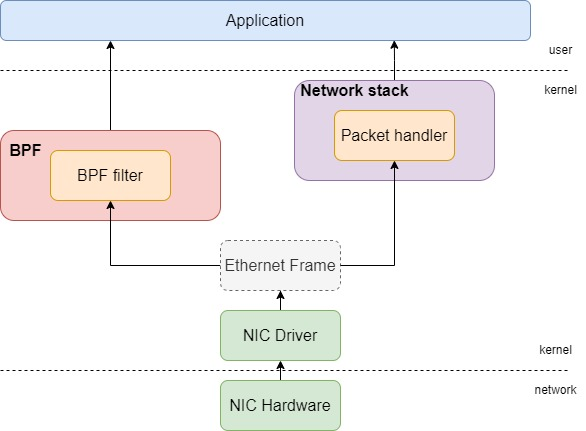
\includegraphics[width=12cm, keepaspectratio=true]{classic_bpf.jpg}
	\caption{Sketch of the functionality of classic BPF}
	\label{fig:classif_bpf}
\end{figure}

Figure \ref{fig:classif_bpf} shows how BPF was integrated in the existing network packet processing by the kernel. After receiving a packet via the Network Interface Controller (NIC) driver, it would first be analysed by BPF filters, which are programs directly developed by the user. This filter decides whether the packet is to be accepted by analysing the packet properties, such as its length or the type and values of its headers. If a packet is accepted, the filter proceeds to decide how many bytes of the original buffer are passed to the application at the user space. Otherwise, the packet is redirected to the original network stack, where it is managed as usual.


\subsection{The BPF virtual machine} \label{section:bpf_vm}
In a technical level, BPF comprises both the BPF filter programs developed by the user and the BPF module included in the kernel which allows for loading and running the BPF filters. This BPF module in the kernel works as a virtual machine\cite{bpf_bsd_origin_bpf_page1}, meaning that it parses and interprets the filter program by providing simulated components needed for its execution, turning into a software-based CPU. Because of this reason, it is usually referred as the BPF Virtual Machine (BPF VM). The BPF VM comprises the following components:
\begin{itemize}
\item \textbf{An accumulator register}, used to store intermediate values of operations.
\item \textbf{An index register}, used to modify operand addresses, it is usually incorporated to optimize vector operations\cite{index_register}.
\item \textbf{An scratch memory store}, a temporary storage.
\item \textbf{A program counter}, used to point to the next machine instruction to execute in a filter program.
\end{itemize}


\subsection{Analysis of a BPF filter program} \label{subsection:analysis_bpf_filter_prog}
As we mentioned in section \ref{section:bpf_vm}, the components of the BPF VM are used to support running BPF filter programs. A BPF filter is implemented as a boolean function:
\begin{itemize}
\item If it returns \textit{true}, the kernel copies the packet to the application.
\item If it returns \textit{false}, the packet is not accepted by the filter (and thus the network stack will be the next to operate it).
\end{itemize}

\begin{figure}[H]
	\centering
	\includegraphics[width=8cm]{cbpf_prog.jpg}
	\caption{Execution of a BPF filter.}
	\label{fig:cbpf_prog}
\end{figure}

Figure \ref{fig:cbpf_prog} shows an example of a BPF filter upon receiving a packet. In the figure, green lines indicate that the condition is true and red lines that it is evaluated as false. Therefore, the execution works as a control flow graph (CFG) which ends on a boolean value\cite{bpf_bsd_origin_bpf_page5}. The figure presents an example BPF program which accepts the following frames:
\begin{itemize}
\item Frames with an IP packet as a payload directed from IP address X.
\item Frames with an IP packet as a payload directed towards IP address Y.
\item Frames belonging to the ARP protocol and from IP address Y.
\item Frames not from the ARP protocol directed from IP address Y to IP address X.
\end{itemize}


\subsection{BPF bytecode instruction format}
In order to implement the CFG to be run at the BPF VM, BPF filter programs are made up of BPF bytecode, which is defined by a new BPF instruction set. Therefore, a BPF filter program is an array of BPF bytecode instructions\cite{bpf_organicprogrammer_analysis}.


\begin{table}[H]
\begin{tabular}{|c|c|c|c|c|}
\hline
& OPCODE & JT & JF & K\\
\hline
BITS & 16 & 8 & 8 & 32\\
\hline
\end{tabular}
\caption{Table showing BPF instruction format. It is a fixed-length 64 bit instruction, the number of bits used by each field are indicated.}
\label{table:bpf_inst_format}
\end{table}

Table \ref{table:bpf_inst_format} shows the format of a BPF bytecode instruction. As it can be observed, it is a compound of:
\begin{itemize}
\item An \textbf{opcode}, similar to assembly opcode, it indicates the operation to be executed.
\item Field \textbf{jt} indicates the offset to the next instruction to jump in case a condition is evaluated as \textit{true}.
\item Field \textbf{jf} indicates the offset to the next instruction to jump in case a condition is evaluated as \textit{false}.
\item Field \textbf{k} is miscellaneous and its contents vary depending on the instruction opcode.
\end{itemize}

\begin{figure}[H]
	\centering
	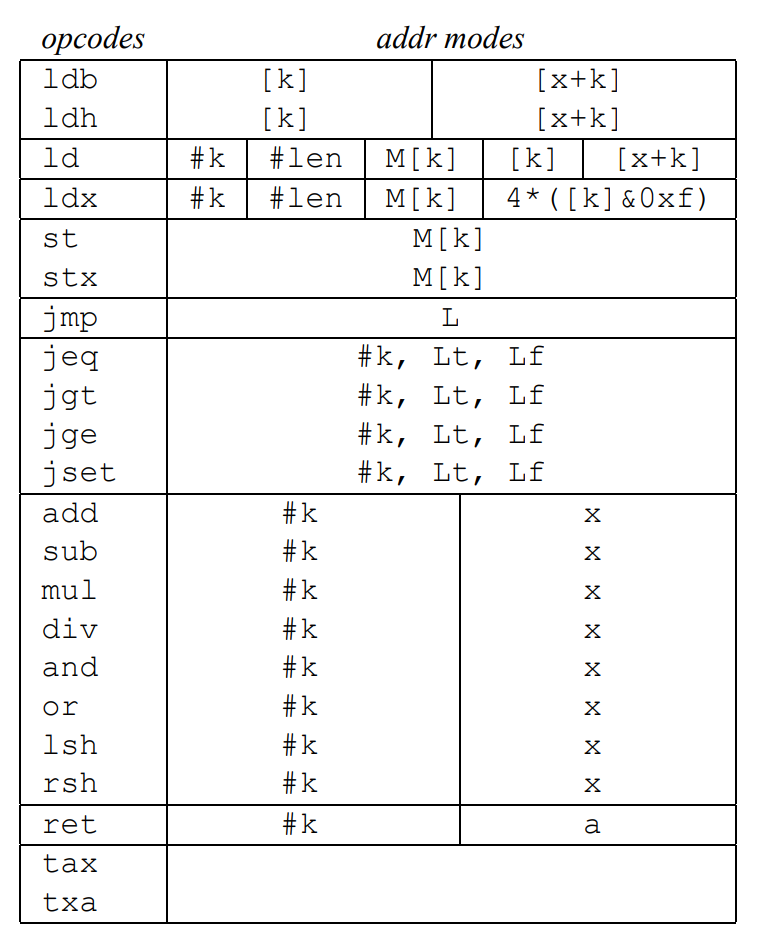
\includegraphics[width=8cm]{bpf_instructions.png}
	\caption{Table of supported classic BPF instructions, as shown by McCanne and Jacobson\cite{bpf_bsd_origin_bpf_page7}}
	\label{fig:bpf_instructions}
\end{figure}

Figure \ref{fig:bpf_instructions} shows how BPF instructions are defined according to the BPF instruction set. As we mentioned, similarly to assembly, instructions include an opcode which indicates the operation to execute, and the multiple arguments defining the arguments of the operation. The table shows, in order by rows, the following instruction types\cite{bpf_bsd_origin_bpf_page8}:
\begin{itemize}
\item Rows 1-4 are \textbf{load instructions}, copying the addressed value into the index or accumulator register.
\item Rows 4-6 are \textbf{store instructions}, copying the accumulator or index register into the scratch memory store.
\item Rows 7-11 are \textbf{jump instructions}, changing the program counter register. These are usually present on each node of the CFG, and evaluate whether the condition to be evaluated is true or not.
\item Rows 12-19 and 21-22 are \textbf{arithmetic and miscellaneous instructions}, performing operations usually needed during the program execution.
\item Row 20 is a \textbf{return instruction}, it is positioned in the final end of the CFG, and indicate whether the filter accepts the packet (returning true) or otherwise rejects it (return false).
\end{itemize}

\begin{figure}[H]
	\centering
	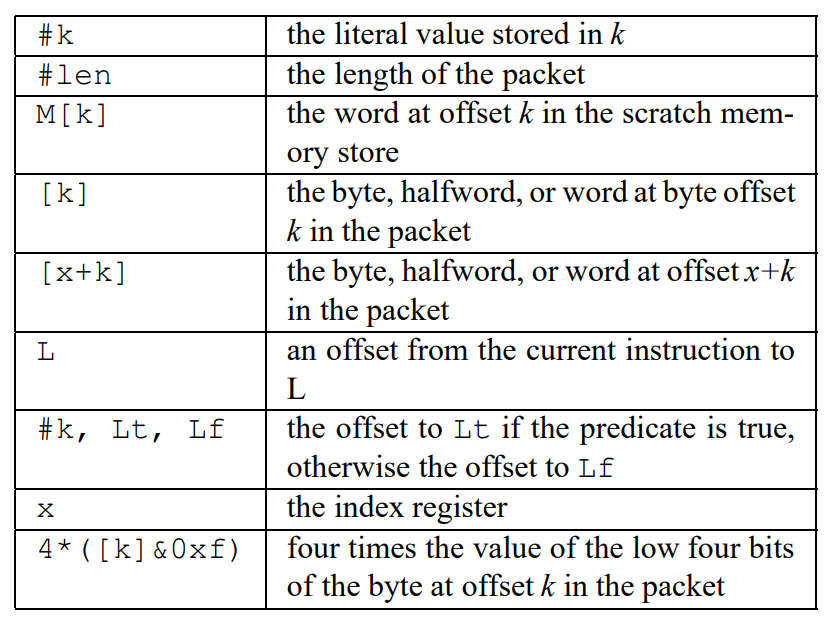
\includegraphics[width=8cm]{bpf_address_mode.png}
	\caption{Table explaining the column address modes in Figure\ref{fig:bpf_instructions}, as shown by McCanne and Jacobson\cite{bpf_bsd_origin_bpf_page8}}
	\label{fig:bpf_address_mode}
\end{figure}

The column \textit{addr modes} in figure \ref{fig:bpf_instructions} describes how the parameters of a BPF instruction are referenced depending on the opcode. The address modes are detailed in figure \ref{fig:bpf_address_mode}. As it can be observed, paremeters may consist of immediate values, offsets to memory positions or on the packet, the index register or combinations of the previous.


\subsection{An example of BPF filter - \textit{tcpdump}}
At the time, by filtering packets before they are handled by the kernel instead of using an user-level application, BPF offered a performance improvement between 10 and 150 times the state-of-the art technologies of the moment\cite{bpf_bsd_origin_bpf_page1}. Since then, multiple popular tools began to use BPF, such as the network tracing tool \textit{tcpdump}\cite{tcpdump_page}.

\textit{tcpdump} is a command-line tool that enables to capture and analyse the network traffic going through the system. It works by setting filters on a network interface, so that it shows the packets that are accepted by the filter. Still today, \textit{tcpdump} uses BPF for the filter implementation. We will now show an example of BPF code used by \textit{tcpdump} to implement a simple filter:

\begin{figure}[H]
	\centering
	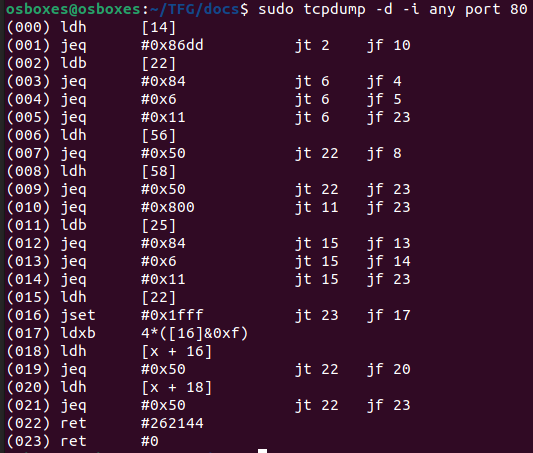
\includegraphics[width=10cm]{tcpdump_example.png}
	\caption{BPF bytecode tcpdump needs to set a filter to display packets directed to port 80.}
	\label{fig:bpf_tcpdump_example}
\end{figure}

Figure \ref{fig:bpf_tcpdump_example} shows how tcpdump sets a filter to display traffic directed to all interfaces (\textit{-i any}) directed to port 80. Flag \textit{-d} instructs tcpdump to display BPF bytecode.

In the example, using the \textit{jf} and \textit{jt} fields, we can label the nodes of the CFG described by the BPF filter. Figure \ref{fig:tcpdump_ex_sol} describes the shortest graph path that a true comparison will need to follow to be accepted by the filter. Note how instruction 010 is checking the value 80, the one our filter is looking for in the port.

\begin{figure}[H]
	\centering
	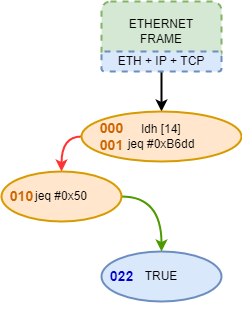
\includegraphics[width=6cm]{cBPF_prog_ex_sol.png}
	\caption{Shortest path in the CFG described in the example of figure \ref{fig:bpf_tcpdump_example} that a packet needs to follow to be accepted by the BPF filter set with \textit{tcpdump}.}
	\label{fig:tcpdump_ex_sol}
\end{figure}

\section{Analysis of modern eBPF}
This section discusses the current state of modern eBPF in the Linux kernel. By building on the previous architecture described in classic BPF, we will be able to provide a comprehensive picture of the underlying infrastructure in which eBPF relies today.

The addition of classic BPF in the Linux kernel set the foundations of eBPF, but nowadays it has already extended its presence to many other components other than traffic filtering. Similarly to how BPF filters were included in the networking module of the Linux kernel, we will now study the necessary changes made in the kernel to support these new program types. Table \ref{table:ebpf_history} shows the main updates that were incorporated and shaped modern eBPF of today.

\begin{table}[H]
\begin{tabular}{|c|c|c|}
\hline
Description & Kernel version & Year\\
\hline
\hline
\textit{BPF}: First addition in the kernel & 2.1.75 & 1997\\
\textit{BPF+}: New JIT assembler & 3.0 & 2011\\
\textit{eBPF}: Added eBPF support & 3.15 & 2014\\
\textit New bpf() syscall & 3.18 & 2014\\
\textit Introduction of eBPF maps & 3.19 & 2015\\
\textit eBPF attached to kprobes & 4.1 & 2015\\
\textit Introduction of Traffic Control & 4.5 & 2016\\
\textit eBPF attached to tracepoints & 4.7 & 2016\\
\textit Introduction of XDP & 4.8 & 2016\\


\hline
\end{tabular}
\caption{Table showing relevant eBPF updates. Note that only those relevant for our research objectives are shown. This is a selection of the official complete table at \cite{ebpf_funcs_by_ver}.}
\label{table:ebpf_history}
\end{table}

As it can be observed in the table above, the main breakthrough happened in the 3.15 version, where Alexei Starovoitov, along with Daniel Borkmann, decided to expand the capabilities of BPF by remodelling the BPF instruction set and overall architecture\cite{brendan_gregg_bpf_book}.

Figure \ref{fig:ebpf_architecture} offers an overview of the current eBPF architecture. During the subsequent subsections, we will proceed to explain its components in detail.

\begin{figure}[H]
	\centering
	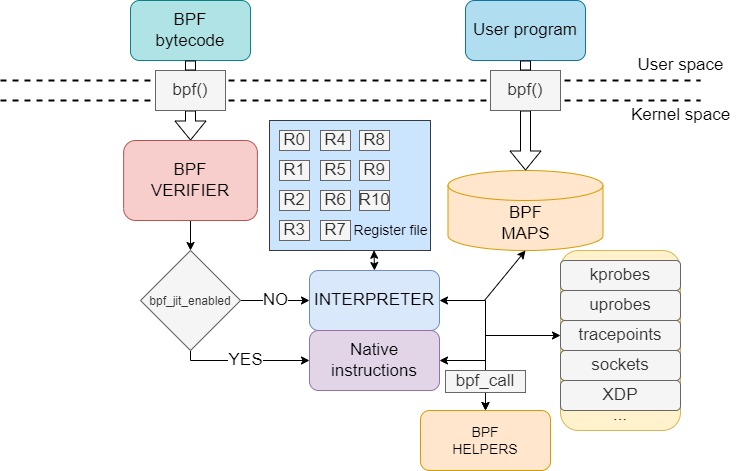
\includegraphics[width=15cm]{ebpf_arch.jpg}
	\caption{Figure showing overall eBPF architecture in the Linux kernel and the process of loading an eBPF program. Based on\cite{brendan_gregg_bpf_book} and \cite{ebpf_io_arch}.}
	\label{fig:ebpf_architecture}
\end{figure}

\subsection{eBPF instruction set} \label{subsection:ebpf_inst_set}
The eBPF update included a complete remodel of the instruction set architecture (ISA) of the BPF VM. Therefore, eBPF programs will need to follow the new architecture in order to be interpreted as valid and executed.

\begin{table}[H]
\begin{tabular}{|c|c|c|c|c|c|}
\hline
& IMM & OFF & SRC & DST & OPCODE \\
\hline
BITS & 32 & 16 & 4 & 4 & 8\\
\hline
\end{tabular}
\caption{Table showing eBPF instruction format. It is a fixed-length 64 bit instruction, the number of bits used by each field are indicated.}
\label{table:ebpf_inst_format}
\end{table}


Table \ref{table:ebpf_inst_format} shows the new instruction format for eBPF programs\cite{ebpf_inst_set}. The new fields are similar to x86\_64 assembly, incorporating the typically found immediate and offset fields, and source and destination registers\cite{8664_inst_set_specs}. Similarly, the instruction set is extended to be similar to the one typically found on x86\_64 systems, the complete list can be consulted in the official documentation\cite{ebpf_inst_set}.
%Should I talk about assembly or this more in detail?

With respect to the BPF VM registers, they get extended from 32 to 64 bits of length, and the number of registers is incremented to 10, instead of the original accumulator and index registers. These registers are also adapted to be similar to those in assembly, as it is shown in table \ref{table:ebpf_regs}.

\begin{table}[H]
\begin{tabular}{|c|c|m{21em}|}
\hline
eBPF register & x86\_64 register & Purpose\\
\hline
r0 & rax & Return value from functions and exit value of eBPF programs\\
r1 & rdi & Function call argument 1\\
r2 & rsi & Function call argument 2\\
r3 & rdx & Function call argument 3\\
r4 & rcx & Function call argument 4\\
r5 & r8 & Function call argument 5\\
r6 & rbx & Callee saved register, value preserved between calls\\
r7 & r13 & Callee saved register, value preserved between calls\\
r8 & r14 & Callee saved register, value preserved between calls\\
r9 & r15 & Callee saved register, value preserved between calls\\
r10 & rbp & Frame pointer for stack, read only\\
\hline
\end{tabular}
\caption{Table showing eBPF registers and their purpose in the BPF VM.\cite{ebpf_inst_set}\cite{ebpf_starovo_slides}.}
\label{table:ebpf_regs}
\end{table}

\subsection{JIT compilation}
We mentioned in subsection \ref{subsection:ebpf_inst_set} that eBPF registers and instructions describe an almost one-to-one correspondence to those in x86 assembly. This is in fact not a coincidence, but rather it is with the purpose of improving a functionality that was included in Linux kernel 3.0, called Just-in-Time (JIT) compilation\cite{ebpf_JIT}\cite{ebpf_JIT_demystify_page13}.

JIT compiling is an extra step that optimizes the execution speed of eBPF programs. It consists of translating BPF bytecode into machine-specific instructions, so that they run as fast as native code in the kernel. Machine instructions are generated during runtime, written directly into executable memory and executed there\cite{ebpf_JIT_demystify_page14}.

Therefore, when using JIT compiling (a setting defined by the variable \textit{bpf\_jit\_enable}\cite{jit_enable_setting}, BPF registers are translated into machine-specific registers following their one-to-one mapping and bytecode instructions are translated into machine-specific instructions\cite{ebpf_starovo_slides_page23}. There no longer exists an interpretation step by the BPF VM, since we can execute the code directly\cite{brendan_gregg_bpf_book_bpf_vm}.

The programs developed during this project will always have JIT compiling active.


\subsection{The eBPF verifier}
We introduced in figure \ref{fig:ebpf_architecture} the presence of the so-called eBPF verifier. Provided that we will be loading programs in the kernel from user space, these programs need to be checked for safety before being valid to be executed.

The verifier performs a series of tests which every eBPF program must pass in order to be accepted. Otherwise, user programs could leak privileged data, result in kernel memory corruption, or hang the kernel in an infinite loop, between others. Therefore, the verifier limits multiple aspects of eBPF programs so that they are restricted to the intended functionality, whilst at the same time offering a reasonable amount of freedom to the developer.

The following are the most relevant checks that the verifier performs in eBPF programs\cite{ebpf_verifier_kerneldocs}\cite{ebpf_JIT_demystify_page17-22}:
\begin{itemize}
\item Tests for ensuring overall control flow safety:
	\subitem No loops allowed (bounded loops accepted since kernel version 5.3\cite{ebpf_bounded_loops}.
	\subitem Function call and jumps safety to known, reachable functions.
\item Tests for individual instructions:
	 \subitem Divisions by zero and invalid shift operations.
	 \subitem Invalid stack access and invalid out-of-bound access to data structures.
	 \subitem Reads from uninitialized registers and corruption of pointers.
\end{itemize}

These checks are performed by two main algorithms:
\begin{itemize}
\item Build a graph representing the eBPF instructions (similar to the one shown in section \ref{subsection:analysis_bpf_filter_prog}. Check that it is in fact a direct acyclic graph (DAG), meaning that the verifier prevents loops and unreachable instructions.
\item Simulate execution flow by starting on the first instruction and following each possible path, observing at each instruction the state of every register and of the stack.
\end{itemize}

\subsection{eBPF maps}


 


















%TODO Talk about the difference between having always on BPF and always on kernel modules


\chapter{Methods??}
%M-> Following the particular TFG we discussed and also others, it looks like the main chapter(s) varies name depending on the TFG topic. Also is there a prefered way to distribute this?


\chapter{Results}


\chapter{Conclusion and future work}




%----------
%	BIBLIOGRAPHY
%----------	

%\nocite{*} % Si quieres que aparezcan en la bibliografía todos los documentos que la componen (también los que no estén citados en el texto) descomenta está lína

\clearpage
\addcontentsline{toc}{chapter}{Bibliography}

\printbibliography



%----------
%	ANEX
%----------	

%M-> Mentioned putting some demos and PoCs here...
%

\chapter* {Appendix A}
\pagenumbering{gobble} % Las páginas de los anexos no se numeran

\chapter* {Appendix B}


\end{document}